\documentclass[12pt]{report}
\usepackage[spanish, activeacute]{babel}
\usepackage[top=2.75cm,bottom=2.50cm,left=3.00cm,right=2.50cm]{geometry}
\usepackage[utf8]{inputenc}  
\usepackage{enumerate}
\usepackage{graphicx}



\begin{document}
	\setlength{\topmargin}{-0.5in}
	\pagestyle{empty}
	\begin{center}
		\textbf{
			\vspace{-0.7em}
			ESCUELA SUPERIOR POLITÉCNICA DEL LITORAL
		}
		\line(1,0){380}\\		
		\scriptsize{FACULTAD DE INGENIERÍA EN ELECTRICIDAD Y COMPUTACIÓN}
	\end{center}

	\begin{center}
		\vspace{2.5em}
		\Huge{\textbf{\\PROYECTO FINAL}}
	\end{center}	

	\begin{center}
		\Huge{\textbf{\\Recopilación de Trabajos II Término 2012	\vspace{1em}}}
	\end{center}
	\begin{center}
		\Huge{\textbf{\\Ana Arias	\vspace{1em}}}
		\\ acarias@espol.edu.ec
	\end{center}
	\begin{center}
		\Huge{\textbf{\\Lenguajes de Programación\vspace{1em}}}
	\end{center}	
	\begin{center}
		\Huge{\textbf{\\Ing. Javier Tibau	\vspace{1em}}}
		\\ jtibau@espol.edu.ec
		\\ jtibau@fiec.espol.edu.ec
	\end{center}	



\chapter*{Agradecimientos}
\addcontentsline{toc}{chapter}{Agradecimientos} 
\markboth{AGRADECIMIENTOS}{AGRADECIMIENTOS} % encabezado 
 
Quiero agradecer a mis compañeros de grupo y compañeros del aula, ya que entre todos compartimos conocimientos y buenas experiencias.
También quiero agradecer a mi profesor de Lenguajes de Programación Ing. Javier Tibau por darnos todos los retos de este semestre.

\chapter*{Resumen} 
\addcontentsline{toc}{chapter}{Resumen} 
\markboth{RESUMEN}{RESUMEN} % encabezado

Este documento contiene las descripciones y experiencias de los proyectos realizados en la materia Lenguajes de Programación dirigida por el Ing. Javier Tibau.

\tableofcontents


%---------------------------------------------------------------------------------------------------------------------------------
%--------------------------------------------------------------GITHUB!------------------------------------------------------
%---------------------------------------------------------------------------------------------------------------------------------
\chapter{Herramienta GitHub\label{capitulouno}}

	\begin{center}
		\begingroup
			
\includegraphics[width=0.27\textwidth]{imagenes_usuario/git.png}
		\endgroup
	\end{center}


	\begingroup
		\large{
			\textbf{
			           \newline
			           \newline
				Experiencias y Anécdotas: GitHub
				\newline
				\newline
			}
		}
	\endgroup
Mi experiencia con GitHub ha sido buena, esta herramienta en verdad mejoró la comunicación en los trabajos con mi grupo; lo que más me agradó es que podemos estar actualizados con respecto a las modificaciones en los archivos que nos tocó hacer de forma grupal, y por lo tanto se evita el compartir documentos frecuentemente a través de otra herramienta y la creación de un sinfín de documentos que contienen en realidad lo mismo.
\newline
\newline	
Considero Github como una red social, ya que podemos estar conectados con nuestros compañeros y compartir información, y además de ser social, es seria ya que a partir de esta herramienta se pueden encontrar trabajos muy interesantes de distintas personas, dicho material puede ser muy útil.
\newline
\newline	
Con respecto a su uso, lo considero sencillo y mecánico; al principio es un poco difícil aprender cómo se utiliza pero después se vuelve costumbre ya que los procedimientos para subir archivos, para crear repositorios, para modificarlos es en realidad muy mecánico.
\newline
Esta herramienta es una buena opción para dar a conocer nuestros trabajos en internet, y seguramente la seguiré utilizando en el futuro.
\newline
\newline
Mi experiencia con Github a lo largo del semestre pasó de ser mala, a regular y finalmente a muy buena. Esto tiene mucho que ver por toda la practica que tuvimos que tener con esta herramienta, ya que la utilizamos en todos los proyectos.
El uso de la herramienta Github se facilitó mucho cuando empecé a utilizar su interfaz.
\newline
	\begin{center}
		\begingroup
			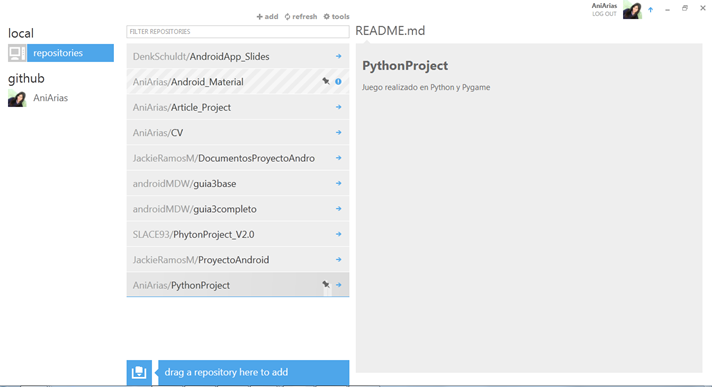
\includegraphics[width=0.8\textwidth]{imagenes_usuario/git2.png}
\newline
\newline
		\endgroup
	\end{center}

	\begin{center}
		\begingroup
			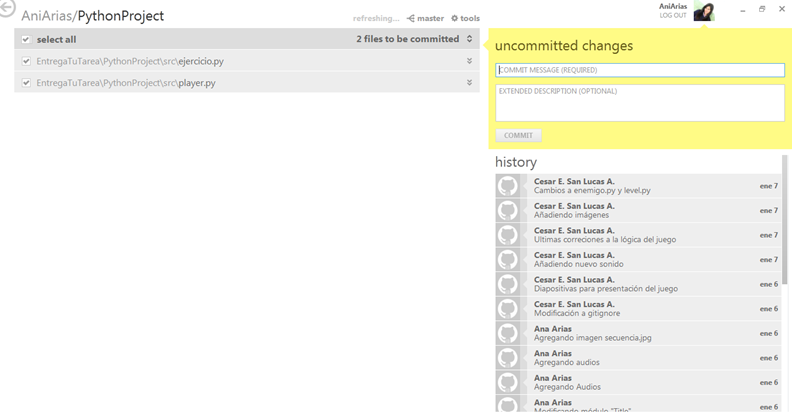
\includegraphics[width=0.8\textwidth]{imagenes_usuario/git3.png}
\newline
\newline
		\endgroup
	\end{center}

La interfaz de Github permite realizar commits de manera mucho mas rápida y mas detallada; me pareció mu interesante la rapidez con que se actualizaban los proyectos cada vez que se modificaba algo.
Recomendaría utilizar la interfaz de GitHub para las personas que recién empiecen a utilizar esta herramienta.
\newline
\newline
Seguiré utilizandola para futuros proyectos y en mi vida profesional.

 \ref{capitulouno}


%---------------------------------------------------------------------------------------------------------------------------------
%--------------------------------------------------------------LATEX------------------------------------------------------
%---------------------------------------------------------------------------------------------------------------------------------


\chapter{Herramienta LateX\label{capitulouno}}

	\begin{center}
		\begingroup
			
\includegraphics[width=0.27\textwidth]{imagenes_usuario/latex.jpg}
		\endgroup
	\end{center}


	\begingroup
		\large{
			\textbf{
				Experiencias y Anécdotas: LaTeX
				\newline
				\newline
			}
		}
	\endgroup

Latex es una buena opción al momento de la creación de documentos de distinto tipo, una herramienta que nos saca de la rutina de los mismos editores de texto que utilizamos a diario; y sin embargo Latex ofrece las mismas características que dichos editores.
\newline	
\newline	
Latex  a pesar de aparentar dificultad, es una herramienta sencilla de utilizar, solo es cuestión de conocer los comandos que permiten editar el formato de nuestro documento.
Otra ventaja de Latex es que existen plantillas para realizar distintos tipos de documentos, estas plantillas facilitan la edición del formato de un texto que quizás no sepamos cómo debería estar formado.
\newline	
\newline	
Como conclusión, el uso de esta herramienta me pareció entretenida y útil, además, fue un reto ya que como programadores debemos ser capaces de adaptarnos a cualquier herramienta.
\newline
\newline		
Existen muchos tutoriales de cómo utilizar Latex, los cuales fueron de mucha ayuda al momento de generar el primer documento que fue el CV, ya que al ser una herramienta nueva, tuve que introducirme al uso de ésta y cuáles son las mejores cualidades que ofrece; para este artículo tengo más experiencia y me costó menos tiempo hacerlo y se me hizo mucho más entretenido.
\newline
Nuestra primera tarea en Latex fue el Curriculum Vitae, al principio el uso de latex, al ser algo nuevo para mi, fue un poco tedioso sin embargo en internet se encuentran muchos tutoriales para crear simpaticos documentos de distintos tipos; se encuentran un sin fin de plantillas que ayudan a empezar a aprender a programar y decorar mucho mejor los documentos que queramos realizar.
Con el tiempo cada vez se hizo mas fácil su uso.
\newline
Lo que me causó mas problema con esta herramienta eran los paquetes que se tenian que instalar para hacer funcionar algunas plantillas, ya que la instalación de estos paquetes a veces era muy rápida y otras veces muy lenta.

La realizacion de mi Curriculum Vitae fue muy útil, ya que éste me ha servido ya en múltiples ocasiones.

El uso de Latex no es cosa del otro mundo, sin embargo existen muchos comandos que sirven para dar formato a nuestros documentos, debemos utilizarlos correctamente ya que si nos olvidamos de cerrar algún bloque de texto o una sentencia, nuestro programa no se compliará de manera exitosa.
\newline
\newline
\newline
\newline
\newline
\newline
\newline
\newline
\newline
\newline
\newline
\newline
\newline
\newline
\newline
\newline
\newline
\newline
\newline
\newline
\newline
\newline
\newline
\newline
\newline
\newline
\newline
\newline

 \ref{capitulouno}


%---------------------------------------------------------------------------------------------------------------------------------
%--------------------------------------------------------------COMIC IT!------------------------------------------------------
%---------------------------------------------------------------------------------------------------------------------------------


\chapter{Proyecto Android \label{capitulodos}}
\begin{center}
		\Huge{\textbf{\\Comic It!	\vspace{1em}}}
\end{center}	


	\begingroup
		\large{
			\textbf{
				Objetivo General
				\newline
				\newline
			}
		}
	\endgroup
	Definir y dar a conocer las funcionalidades y los requerimientos que tendrá el proyecto para la materia Lenguajes de Programación de la Escuela Superior Politécnica del Litoral. 
\newline
\newline
Constrastar y relatar las experiencias vividas con GitHub y LaTeX.
	\vspace{4em}
	\newline
	\begingroup
		\large{
			\textbf{
				Objetivos Específicos
				\newline
			}
		}
	\endgroup
		\begin{enumerate}[(a)]%for small alpha-characters within brackets.
		\item Conocer las funcionalidades de la nueva aplicación para Android: Comic It!.
		\item Describir cada una de las funcionalidades que tendrá la aplicación.
		\item Especificar quiénes serán los usuarios finales de la aplicación.
		\item Presentar ciertas características que tendrá la aplicación final.
		\item Exponer experiencias con la instalación/utilización de GitHub y LaTex.
		\item Relatar anécdotas con la instalación/utilización de GitHub y LaTex.
		\end{enumerate}
	
	
\newpage
	\begingroup
		\large{
			\textbf{
				Descripción
				\newline
				\newline
			}
		}
	\endgroup

	%
	%Descripcion
	%
``Comic It!'' es una nueva aplicación para disposivos móviles que utilizan como sistema operativo Android. El nombre representa completamente a este nuevo software, puesto que será diseñado para crear historietas.
\newline
\newline
``Comic It!'' tendrá como usuarios a personas que les gusta tomar fotos y conservar recuerdos de los momentos divertidos que viven diariamente.
\newline
\newline
Con plantillas para colocar sus fotos, burbujas de diálogo e imágenes predeterminadas, el usuario quedará satisfecho cuando obtenga su obra final en su dispositivo.
\newline
\newline
Esta historieta relatará de una manera divertida, humorística y muy colorida exactamente lo que el usuario ha vivido o haya querido inventar para su uso personal.
	\newline
	\newline
	\newline
	\begingroup
		\large{
			\textbf{
				Funcionalidades
				\newline
				\newline
			}
		}
	\endgroup
	%
\newline
Comic It! cuenta con una variedad de funcionalidades que el usuario puede usar de manera rápida y dinámica utilizando 				fotos tomadas directamente de la CÁMARA o de la GALERÍA FOTOGRÁFICA .
\newline
\newline
El usuario tendrá la opción de crear un collage tipo caricatura  con fotografías de la galería de fotos del celular en una plantilla escogida de una LISTA DE PLANTILLAS proporcionadas por la aplicación.
\newline
\newline
Comic It! cuenta con una LISTA DE ÍCONOS básicos y personalizados que permitirán al usuario crear imágenes más reales y divertidas.	
\newline
\newline	
Además de íconos, el usuario tendrá una LISTA DE TEXTOS divertidos para darle mas creatividad a las escenas que esté creando.
\newline
\newline
Proporciona una lista con varios formatos de BURBUJAS DE DIALOGO, de las cuales el usuario puede escoger las que más se ajuste a su necesidad. El usuario podrá EDITAR EL TEXTO dentro de la burbuja de dialogo que haya escogido, convirtiendo a los miembros de 		la fotografía en auténticos personajes.
\newline
\newline
Al terminar de crear caricaturas, se podrán guardar en la galería fotográfica en distintos FORMATOS.

\newpage
	\begingroup
		\large{
			\textbf{
				Ilustración	
				\newline
				\newline
			}
		}
	\endgroup
Este es un pequeño vistazo a como se espera que sea la aplicación, resaltando sus partes más importantes:
	\newline

	\begin{center}
		\begingroup
			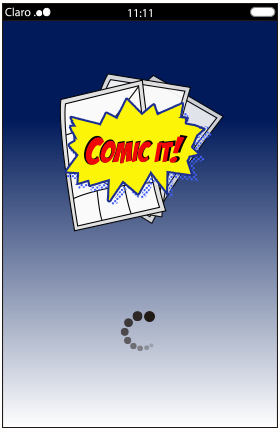
\includegraphics[width=0.19\textwidth]{imagenes_usuario/demo1.jpg}
		\endgroup
		\begingroup
			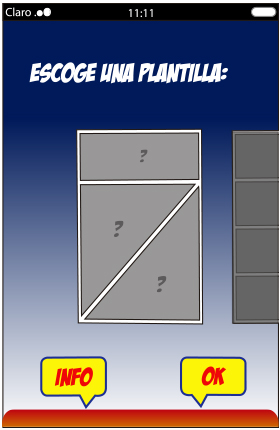
\includegraphics[width=0.19\textwidth]{imagenes_usuario/demo2.jpg}
		\endgroup
		\begingroup
			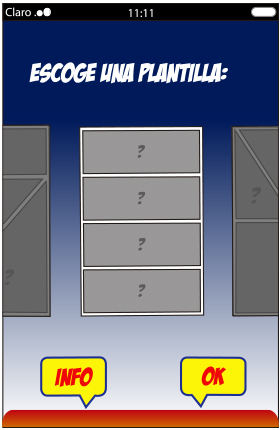
\includegraphics[width=0.19\textwidth]{imagenes_usuario/demo3.jpg}
		\endgroup
		\begingroup
			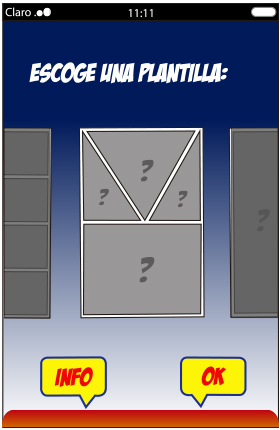
\includegraphics[width=0.19\textwidth]{imagenes_usuario/demo4.jpg}
		\endgroup
		\begingroup
			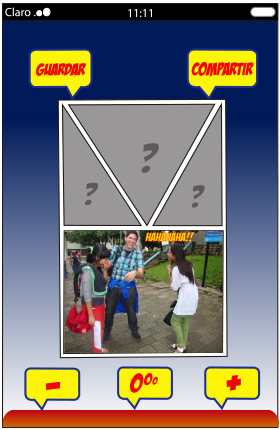
\includegraphics[width=0.19\textwidth]{imagenes_usuario/demo5.jpg}
		\endgroup
	\end{center}

\begingroup
			\vspace{3mm}
		\endgroup
Se observa la imagen inicial de la aplicación, seguido de las pantallas de selección de plantillas. Luego, puede verse un bosquejo de la aplicación en su parte más importante: La edición de la historieta.
 \newline
 \newline
En la parte superior, se tienen los botones 'Guardar' y 'Compartir'. Guardar, como su nombre lo indica, permitiría guardar la aplicación en la librería de imágenes del smartphone. 'Compartir' permitiría mostrar la historieta finalizada en las redes sociales, Twitter y Facebook.
 \newline
 \newline
En la parte inferior se observan los botones '-', '+'  y el botón de selección de burbujas. Los dos primeros botones servirían para redimensionar las burbujas o íconos en pantalla.

\newpage
\begin{center}	
	\vspace{1em}
		\Huge{\textbf{\\Manual de Usuario	\vspace{1em}}}
	\end{center}	


\begingroup
		\large{
			\textbf{
				Cargando la Cámara...
				\newline
				\newline
			}
		}
	\endgroup
Espere mientras la aplicación ComicIt! es cargada completamente.


	\begin{center}
		\begingroup
			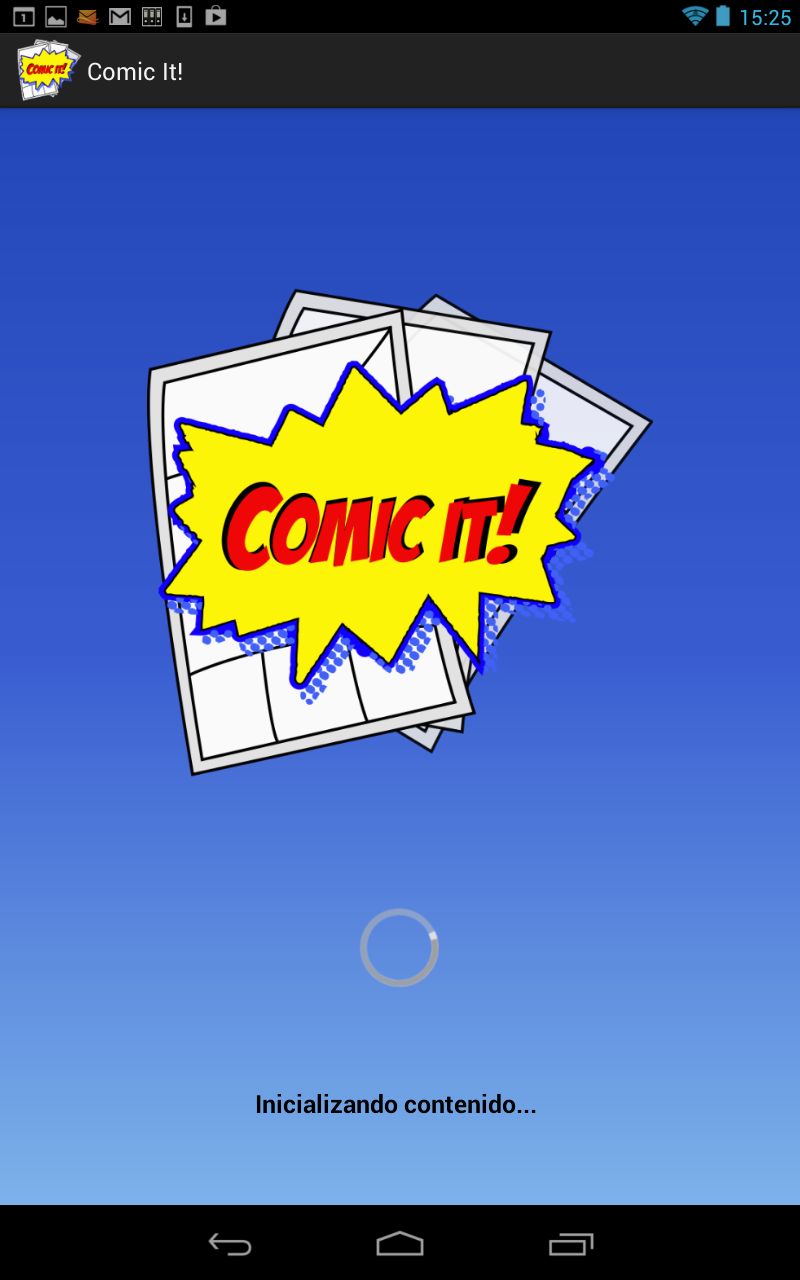
\includegraphics[width=0.27\textwidth]{imagenes_usuario/cargar.png}
		\endgroup
	\end{center}


\begingroup
		\large{
			\textbf{
				Escogiendo Plantilla...
				\newline
				\newline
			}
		}
	\endgroup
Al abrir la aplicación se encontrarán las opciones de plantillas, de las cuales el usuario puede escoger la que desee según el tipo de caricatura que desee crear; estas plantillas contienen la opción de colocar 5 imágenes, colocadas en distintas posiciones según el diseño de la plantilla.
				\newline
				\newline
	\begin{center}
		\begingroup
			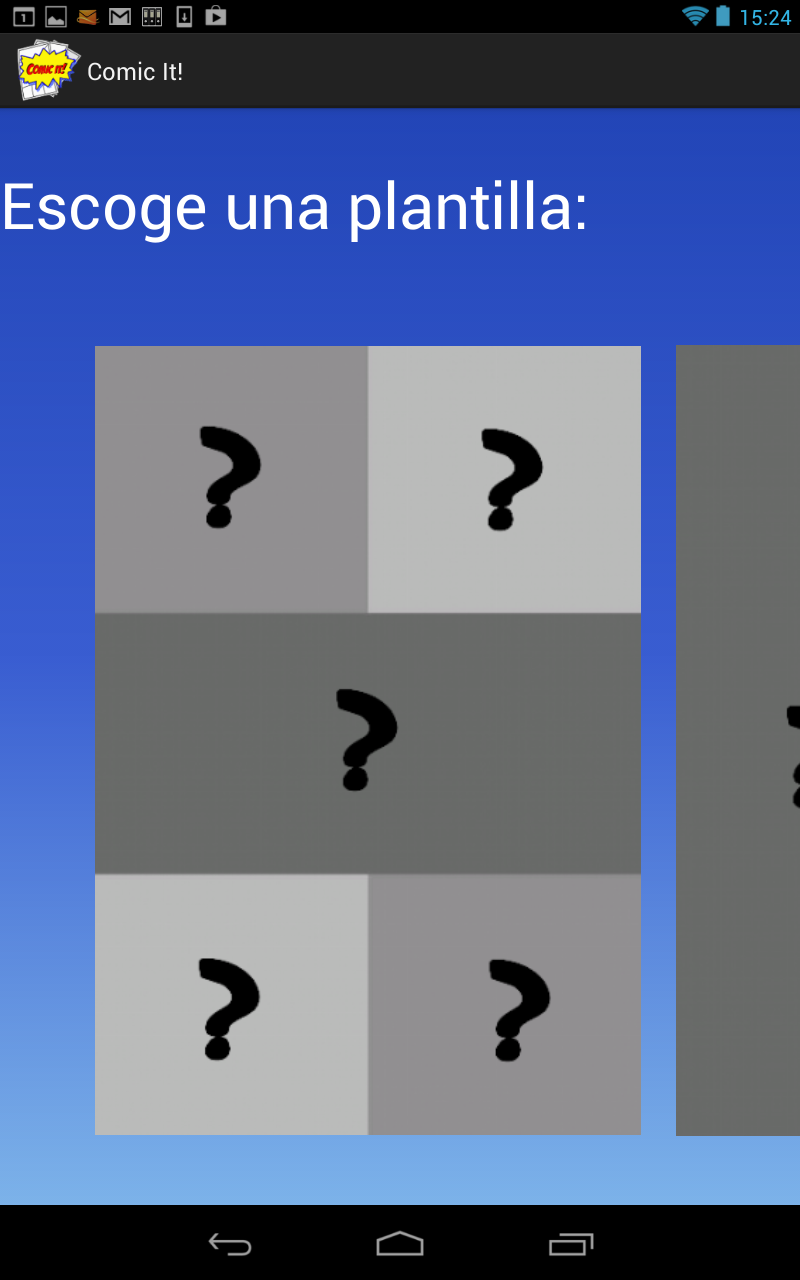
\includegraphics[width=0.24\textwidth]{imagenes_usuario/plantillas.png}
		\endgroup
	\end{center}


\begingroup
		\large{
			\textbf{
				Llenando Plantilla con fotos...
				\newline
				\newline
			}
		}
	\endgroup
Al darle un click a la plantilla que se desea escoger se abrirá una ventana en la cual la plantilla escogida saldrá en toda la pantalla. El usuario podrá empezar a crear su caricatura!
Para poder colocar fotos en los recuadros de la plantilla, el usuario tendrá que darle click al recuadro que desea rellenar con fotos tomadas ya sea desde la cámara o la galería de fotos del celular
\newline
\newline
	\begin{center}
		\begingroup
			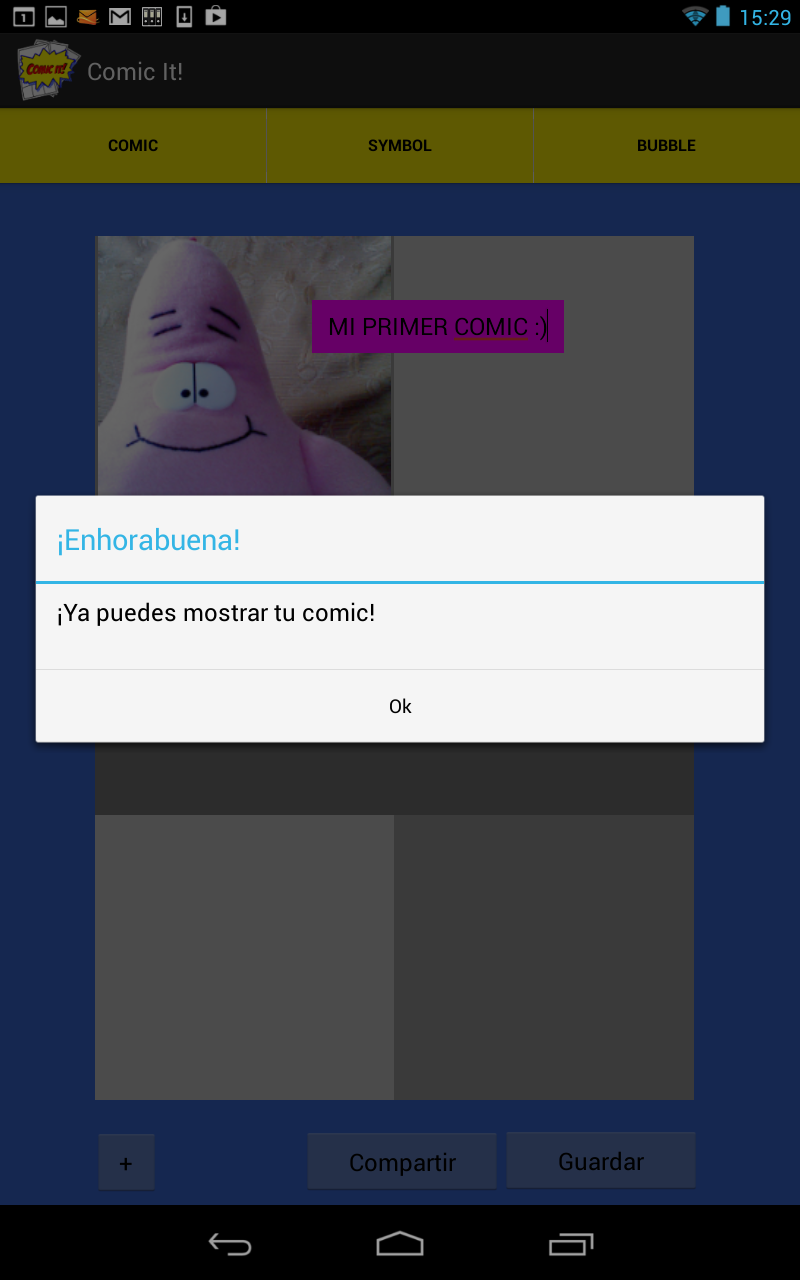
\includegraphics[width=0.27\textwidth]{imagenes_usuario/camara.png}

		\endgroup
	\end{center}


\begingroup
		\large{
			\textbf{
				Usando la Cámara...
				\newline
				\newline
			}
		}
	\endgroup
Si se escoge la opción cámara, automáticamente aparecerá la cámara del celular, de la cual se tomará la foto deseada.
\newline
\newline
\newline
	\begin{center}
		\begingroup
			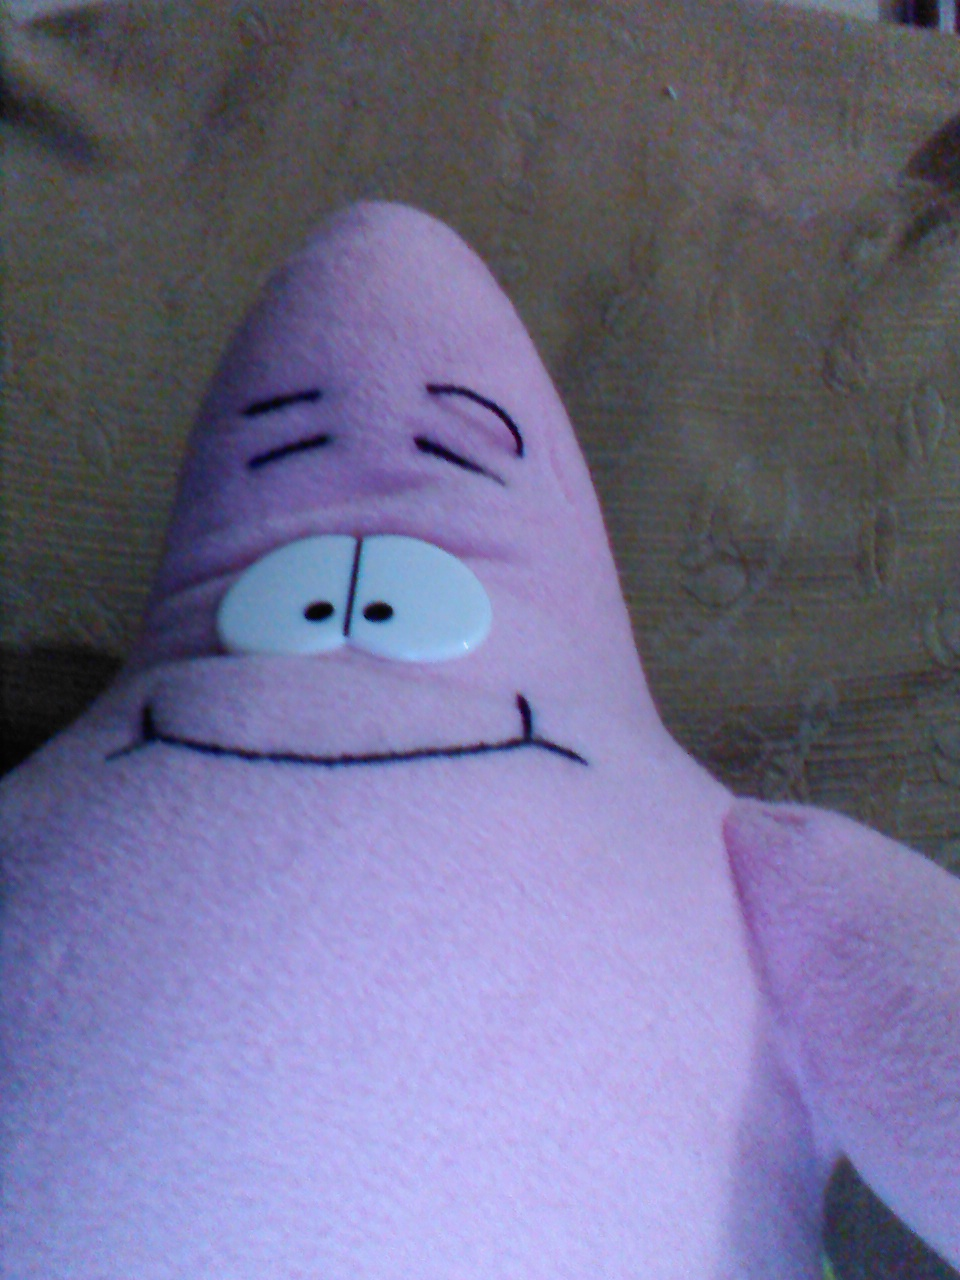
\includegraphics[width=0.27\textwidth]{imagenes_usuario/foto.jpg}
		\endgroup
	\end{center}



\begingroup
		\large{
			\textbf{
				Accediendo a la galería...
				\newline
				\newline
			}
		}
	\endgroup
Si por el contrario se escoge la galería de fotos, se abrirá automáticamente la galería fotográfica del celular, en la que se deberá buscar la foto deseada y escogerla.
\newline
\newline
	\begin{center}
		\begingroup
			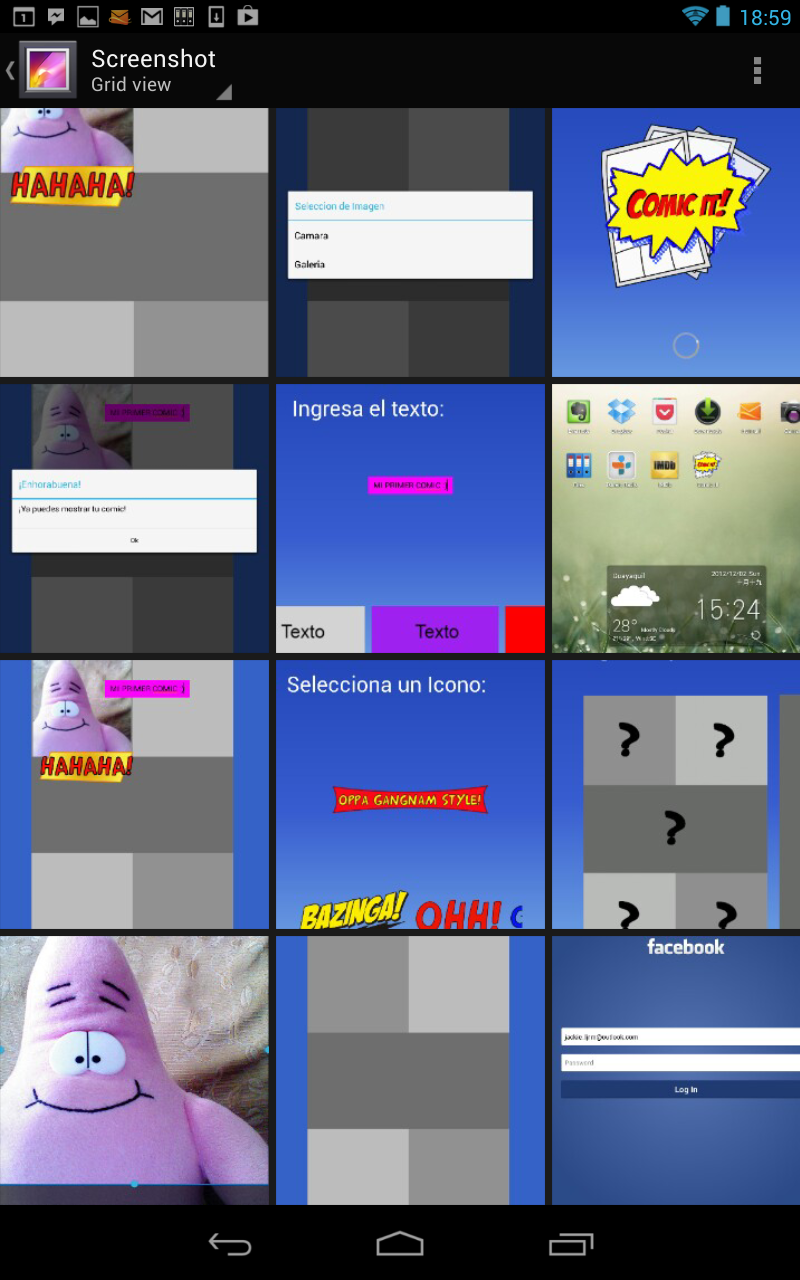
\includegraphics[width=0.27\textwidth]{imagenes_usuario/galeria.png}
		\endgroup
	\end{center}


\begingroup
		\large{
			\textbf{
				Recortando foto...
				\newline
				\newline
			}
		}
	\endgroup
Una vez obtenida la foto deseada, se creará automáticamente la opción para recortar dicha foto, y así determinar el rango de imagen que se desea de la foto tomada.
\newline
\newline
\newline
	\begin{center}
		\begingroup
			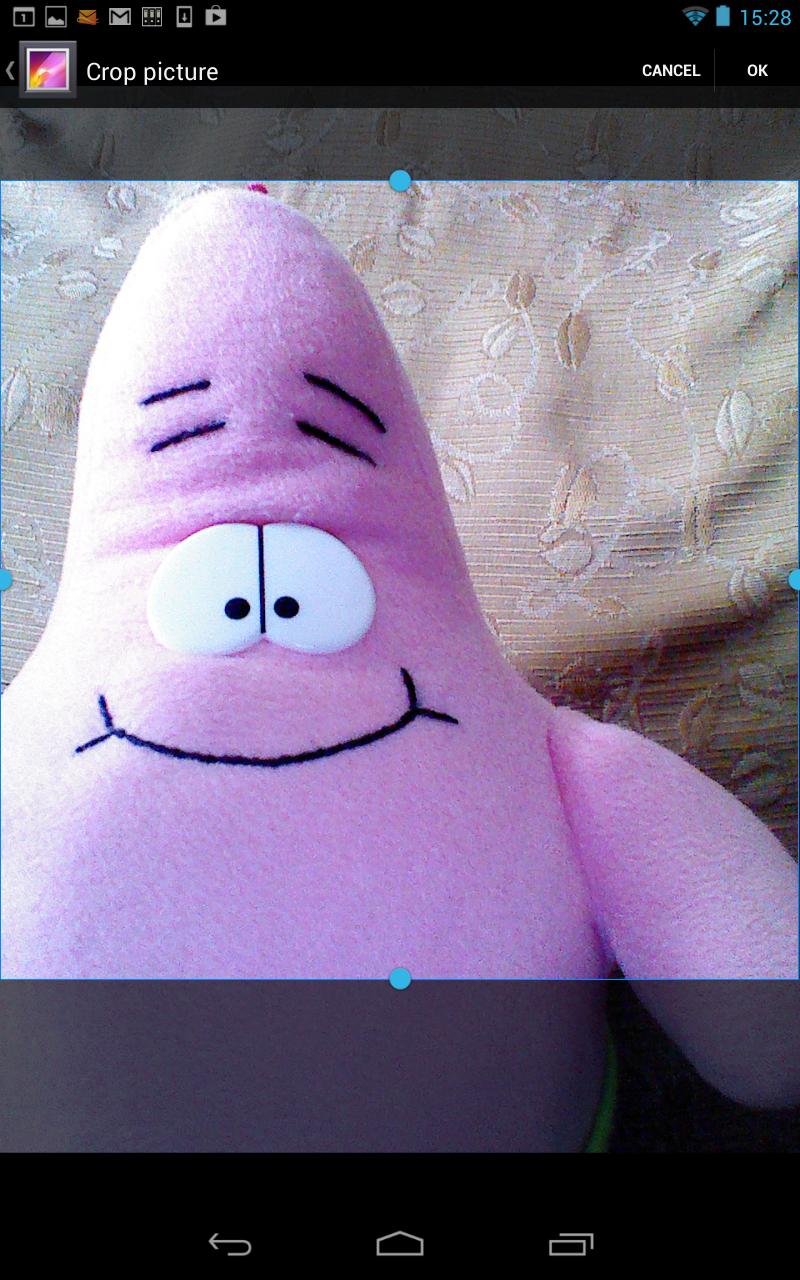
\includegraphics[width=0.27\textwidth]{imagenes_usuario/crop.png}
		\endgroup
	\end{center}


Luego de recortar la imagen y aceptar, la imagen obtenida y recortada se colocará en el recuadro que escogimos. Se debe repetir el proceso para los demás recuadros en la plantilla.
\newline
	\begin{center}
		\begingroup
			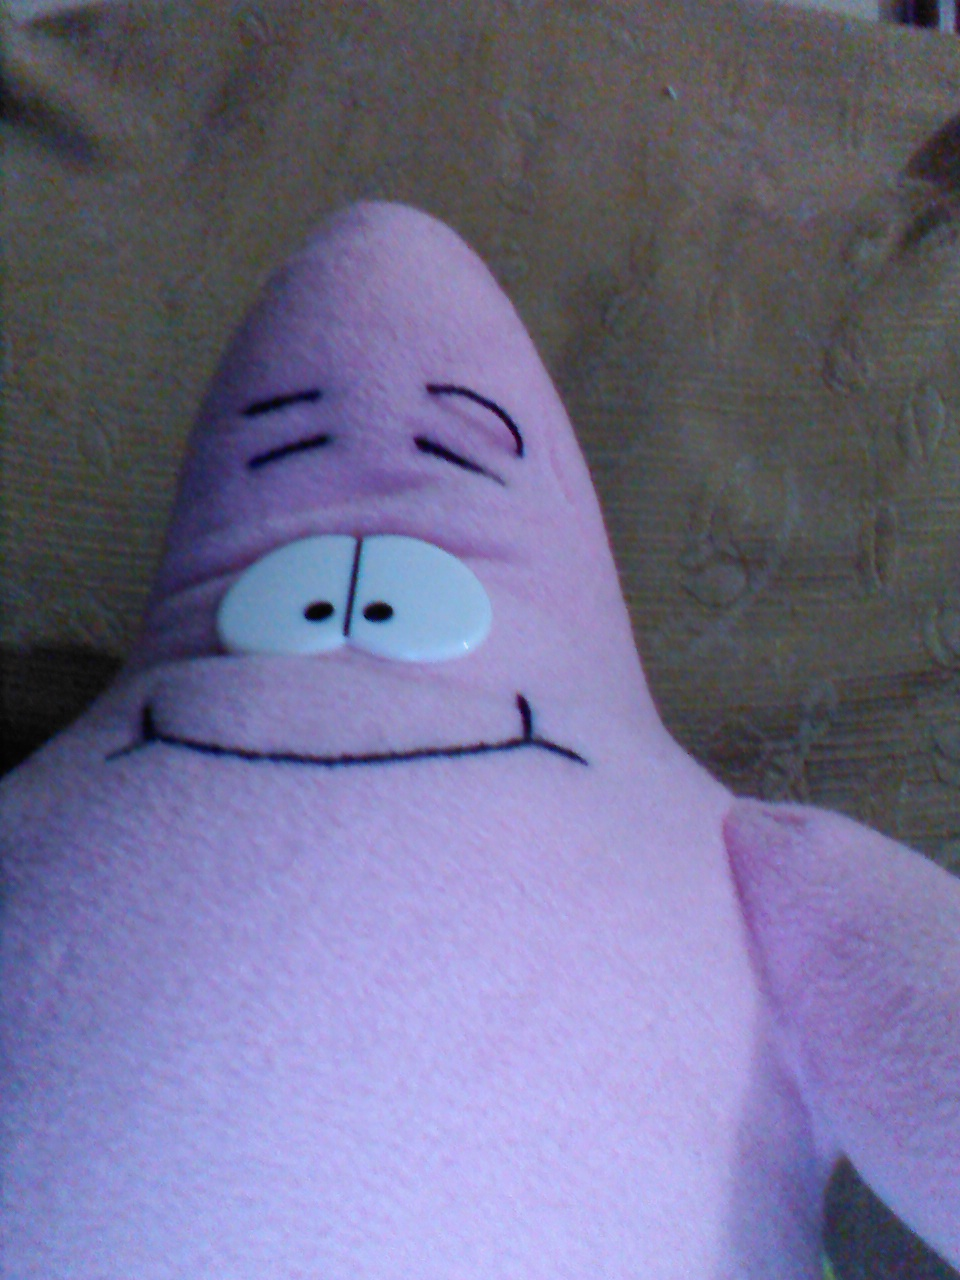
\includegraphics[width=0.27\textwidth]{imagenes_usuario/foto.jpg}
		\endgroup
	\end{center}


El usuario tiene la opción de cambiar la foto de los recuadros cuantas veces desee.
La plantilla está lista para convertirse en una caricatura.
El usuario tendrá las opciones de agregar a su plantilla, íconos con textos divertidos  y con diseños propios de los autores de Comic It!
\newline
\newline

\begingroup
		\large{
			\textbf{
				Iconos...
				\newline
				\newline
			}
		}
	\endgroup
Al escoger la opción de Symbols en los Tabs superiores, se abrirá una ventana que muestre la variedad de símbolos que el usuario puede escoger según lo que más se ajuste al tipo de caricatura que esté creando. Una vez escogido el símbolo, éste aparecerá en la plantilla que contiene las fotos anteriormente escogidas.
	\begin{center}
		\begingroup
			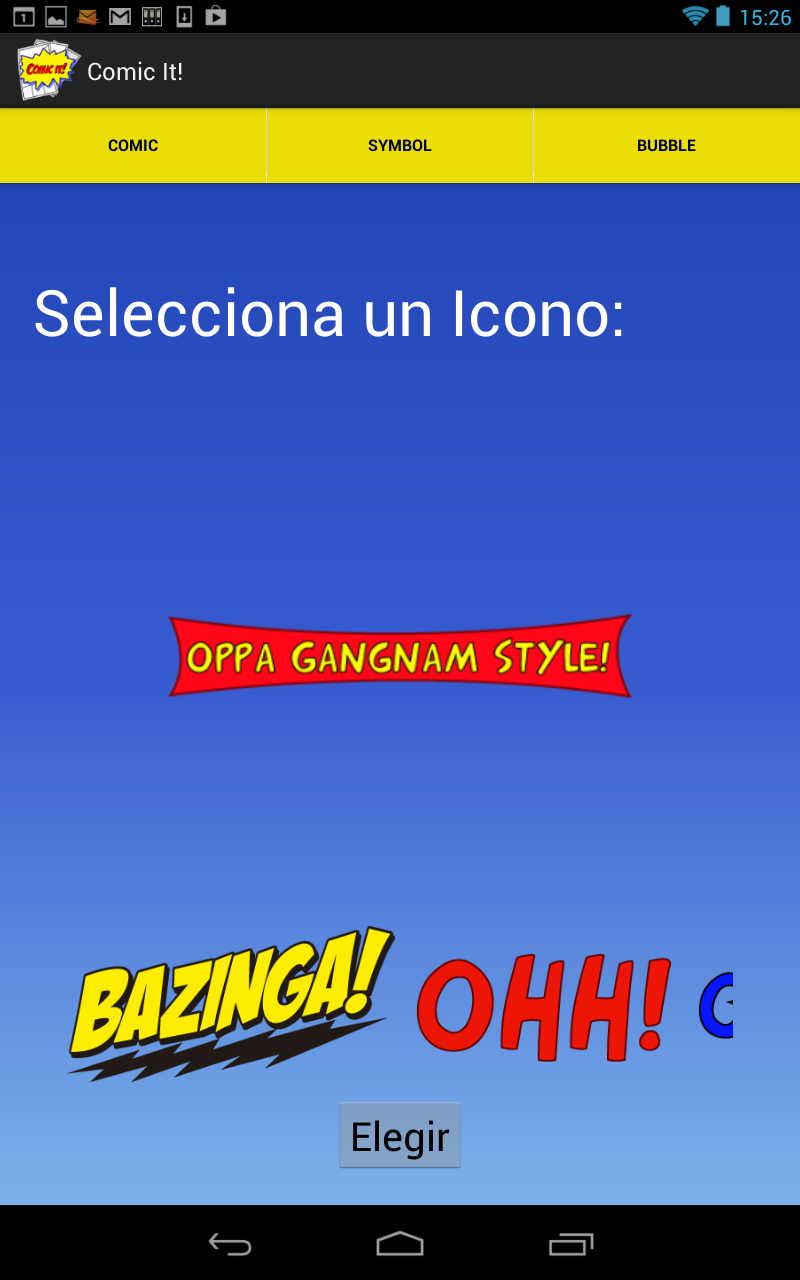
\includegraphics[width=0.30\textwidth]{imagenes_usuario/iconos.png}
		\endgroup
	\end{center}


\begingroup
		\large{
			\textbf{
				Burbujas...
				\newline
				\newline
			}
		}
	\endgroup
El usuario tendrá la opción de arrastrar el ícono escogido en cualquier espacio de la plantilla. Podrá repetir el proceso con el número de íconos que desee colocar en su caricatura.
Al escoger la opción de Burbujas en los Tabs superiores, se abrirá una ventana que muestre la variedad de colores de burbujas que el usuario puede escoger según lo que más se ajuste al tipo de caricatura que esté creando. Una vez escogido el color de la burbuja, el usuario podrá escribir el texto que desee que esté en el interior de dicha burbuja; al terminar este proceso, la burbuja editada (con su correspondiente texto y color) aparecerá en la plantilla que contiene las fotos anteriormente escogidas.

	\begin{center}
		\begingroup
			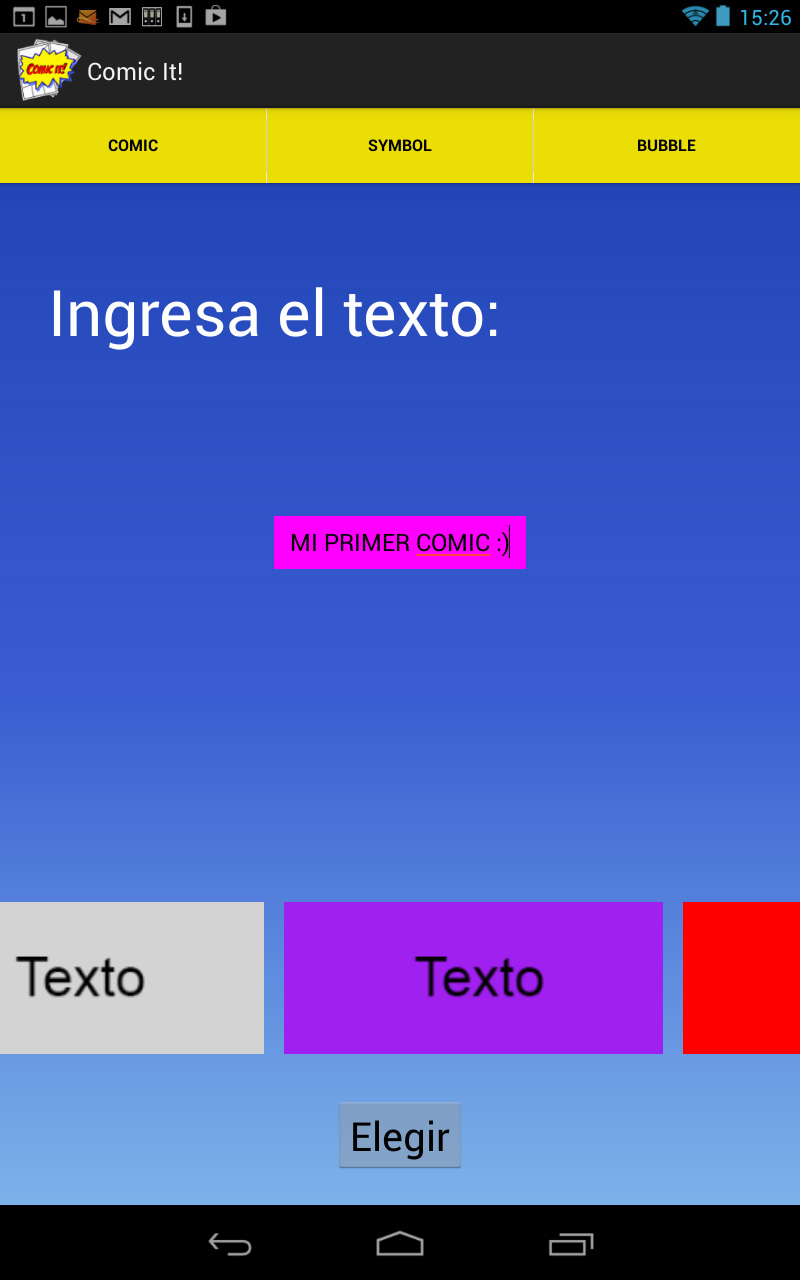
\includegraphics[width=0.27\textwidth]{imagenes_usuario/texto.png}
		\endgroup
	\end{center}

%--------------------------------------------------------------------------------------------------------------------


\begingroup
		\large{
			\textbf{
				Colocando imágenes...
				\newline
				\newline
			}
		}
	\endgroup
El usuario tendrá la opción de arrastrar la burbuja escogida en cualquier espacio de la plantilla. Podrá repetir el proceso con el número de burbujas que desee colocar en su caricatura.
\newline


	\begin{center}
		\begingroup
			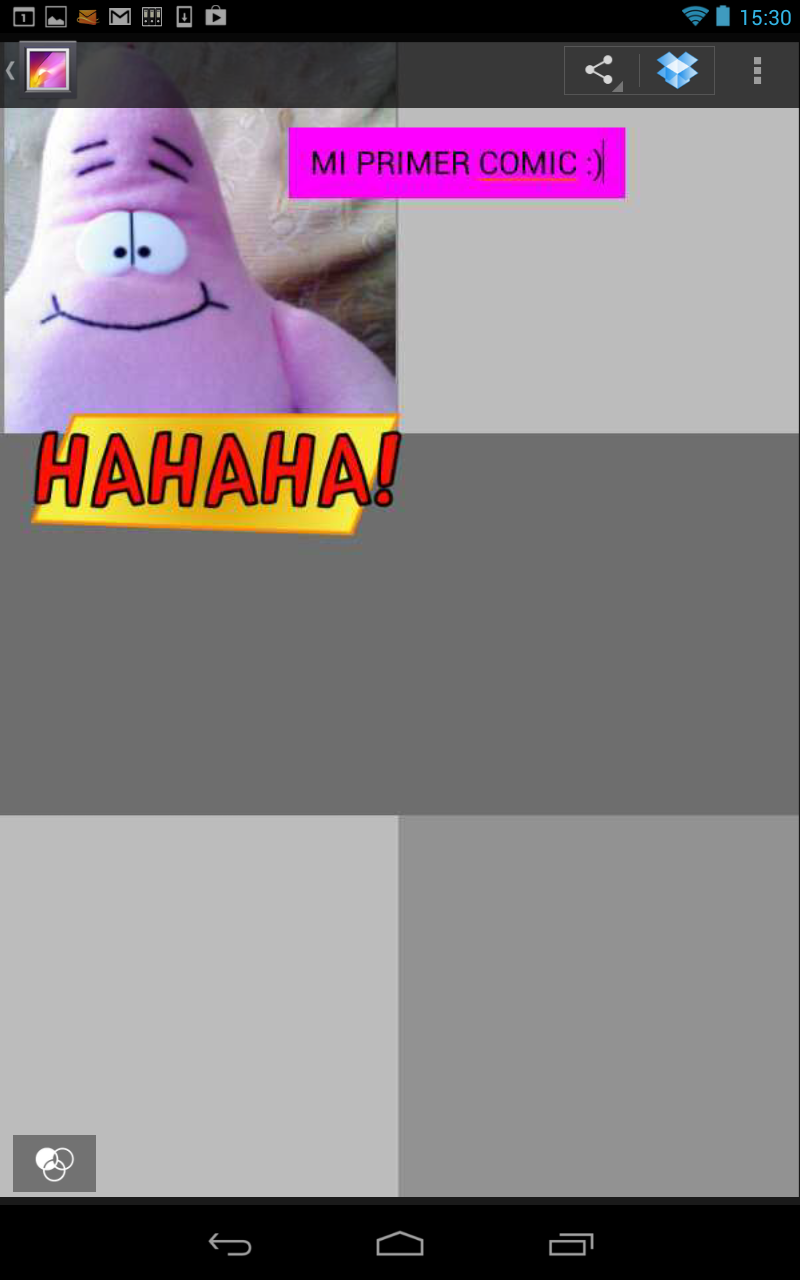
\includegraphics[width=0.27\textwidth]{imagenes_usuario/comic.png}
		\endgroup
	\end{center}

%--------------------------------------------------------------------------------------------------------------------


\begingroup
		\large{
			\textbf{
				Compartiendo nuestra caricatura
				\newline
				\newline
			}
		}
	\endgroup
Presionar el botón guardar para que la caricatura se guarde en la memoria del celular.
Hoy en día las redes sociales son muy utilizadas en cualquier actividad que realicemos. ¿Por qué no compartir nuestra experiencia con amigos o familiares?
Por esto Comic It! permite compartir tu experiencia en Facebook.
\newline

	\begin{center}
		\begingroup
			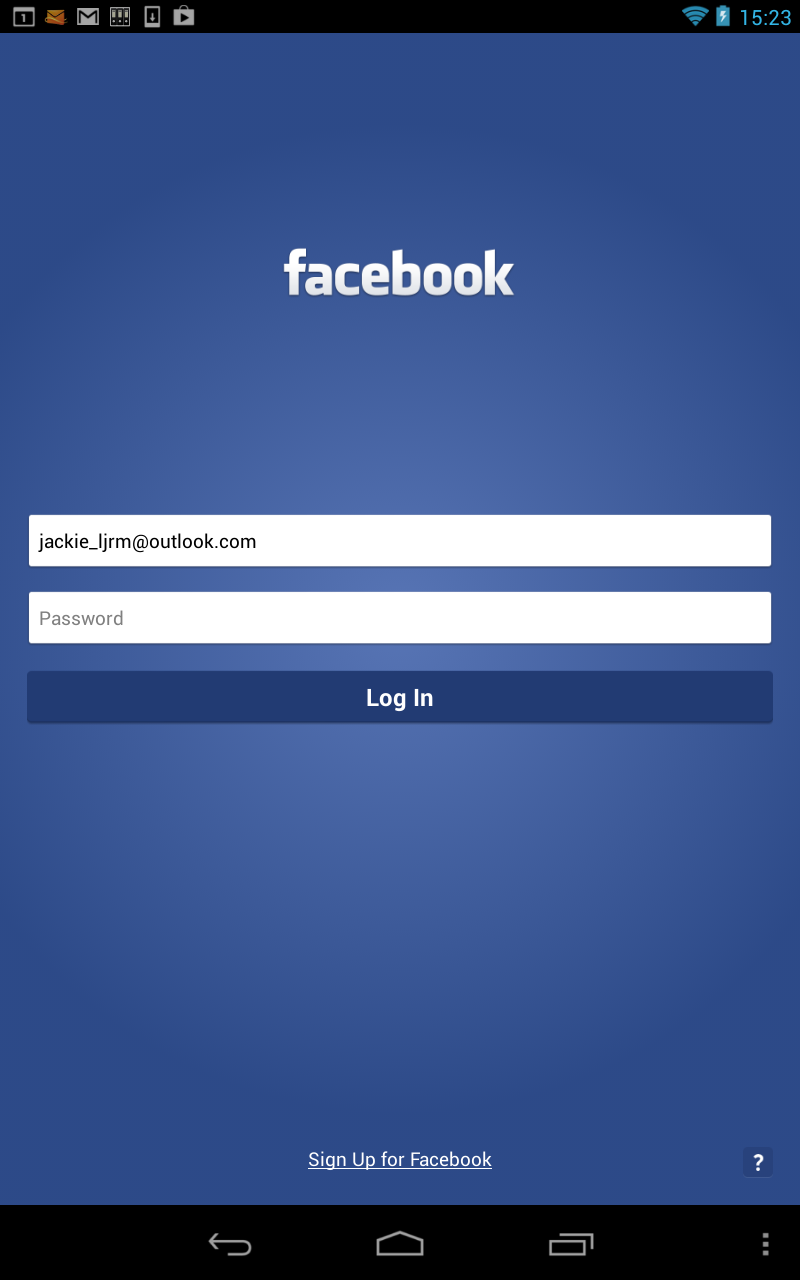
\includegraphics[width=0.27\textwidth]{imagenes_usuario/face.png}

		\endgroup
	\end{center}


 \ref{capitulodos}













\end{document}